% Ensure xcolor options are set before any class/package loads it
\PassOptionsToPackage{usenames,dvipsnames}{xcolor}
\documentclass{beamer}
\usepackage[unilu,en]{collegeBeamer}
\usepackage[backend=biber]{biblatex}
%\usepackage[usenames,dvipsnames]{xcolor}
\setbeamertemplate{footline}[frame number]
\usepackage{graphicx}
\usepackage{tikz}
\usetikzlibrary{calc, arrows.meta, intersections, patterns, positioning, shapes.misc, shapes.geometric, fadings, through, decorations.pathreplacing}
\usepackage{pgfplots}
\pgfplotsset{compat=1.18}
\usepackage{etoolbox}
\usepackage{booktabs}
\usepackage{fontawesome5}

\addbibresource{references.bib}

% meta-data
\title{GraphSAGE}
\subtitle{Inductive Representation Learning\\on Large Graphs}
\author{Thomas Gantz\\Alberto Finardi\\Tommaso Crippa\\Jan Marxen}
\date{\today}
\themecolor{50,50,50}

% document body
\begin{document}

\maketitle

%-----------------------------------------------------------------------
\section{Introduction}
%-----------------------------------------------------------------------

\begin{frame}{Graph Prediction Tasks}
    \begin{columns}
        \begin{column}{0.55\textwidth}
            \textbf{Primary focus:} Node-level prediction — predict properties of individual nodes (classification, regression).
            
            \vspace{10pt}
            \begin{itemize}
                \item \textbf{Node-level (focus):} Predict node attributes or labels using features and neighbor information.
                \item \textbf{Edge-level:} Predict relationships between node pairs (link prediction, edge classification).
                \item \textbf{Graph-level:} Predict properties of whole graphs (e.g., molecule properties).
            \end{itemize}
        \end{column}
        \begin{column}{0.42\textwidth}
            \centering
            \includegraphics[width=1.2\textwidth]{img/gnn_intro_node_level_task.png}
        \end{column}
    \end{columns}
\end{frame}

\begin{frame}{What is a Graph Neural Network?}

    \vspace{4pt}
    \textbf{A learnable transformation} on graph attributes that:
    \begin{itemize}
        \item Updates node/edge/graph features using \textbf{neural networks}
        \item \textbf{Respects graph structure} by aggregating information from neighbors
        \item Is \textbf{permutation invariant} (order of nodes doesn't matter)
    \end{itemize}
    
    \vspace{5pt}
    \centering
    \includegraphics[width=0.75\textwidth]{img/gnn_intro_whatisgnn.png}
\end{frame}

\begin{frame}{Message Passing: The Core Idea}
    \textbf{Three steps repeated at each layer:}
    \begin{enumerate}
        \item \textbf{Gather:} Collect embeddings from neighboring nodes
        \item \textbf{Aggregate:} Combine neighbors' info (sum / mean / max)
        \item \textbf{Update:} Apply learned transform using the aggregated vector
    \end{enumerate}
    
    \vspace{6pt}
    \centering
    \includegraphics[width=0.85\textwidth]{img/gnn_intro_message_passing.png}
\end{frame}

\begin{frame}{Message Passing: Notation}
    \begin{block}{Message Passing Equation}
        \centering
        $h_v^{(k)} = \sigma\left( W \cdot \left[ h_v^{(k-1)} \, , \, \mathrm{AGG}\left(\{ h_u : u \in N(v) \}\right) \right] \right)$
    \end{block}
    
    \vspace{4pt}
    \begin{columns}
        \begin{column}{0.48\textwidth}
            \small
            \begin{itemize}
                \item $h_v^{(k)}$ — Node $v$ repr. at layer $k$
                \item $h_u$ — Neighbor node $u$ repr.
                \item $N(v)$ — Neighbors of $v$
                \item $k$ — Layer index (hops)
            \end{itemize}
        \end{column}
        \begin{column}{0.48\textwidth}
            \small
            \begin{itemize}
                \item $\mathrm{AGG}(\cdot)$ — Aggregator (mean, sum, max)
                \item $W$ — Learnable weight matrix
                \item $\sigma$ — Activation (ReLU, tanh)
            \end{itemize}
        \end{column}
    \end{columns}
\end{frame}

\begin{frame}{Before GraphSAGE: The Problem}
    \textit{Let's audit the limitations of existing approaches...}
    
    \vspace{12pt}
    \begin{itemize}
        \item \textbf{DeepWalk / node2vec:} Transductive: embed every node; new nodes need full retraining.\\
              \hspace{1em}{\small \textcolor{gray}{$\triangleright$ Not GNNs — random-walk based embeddings, no message passing}}
        \item \textbf{GCNs:} Often require access to the full graph during training/inference; can be costly to scale.\\
              \hspace{1em}{\small \textcolor{gray}{$\triangleright$ GNNs — but transductive: fixed node set at training}}
        \item \textbf{Result:} No compact parametric function to generate embeddings for unseen nodes.
    \end{itemize}
    
    \vspace{12pt}
    \textit{This motivates GraphSAGE's key insight...}
\end{frame}

%-----------------------------------------------------------------------
\section{The Key Insight}
%-----------------------------------------------------------------------

\begin{frame}{The Key Insight}
    \centering
    \vspace{5pt}
    
    {\Large \textbf{Don't learn embeddings for each node...}}
    
    \vspace{10pt}
    
    {\Large \textcolor{orange}{\textbf{Learn a FUNCTION that generates embeddings}}}
    
    \vspace{8pt}
    
    \textit{By sampling \& aggregating neighborhood features}
    
    \vspace{8pt}
    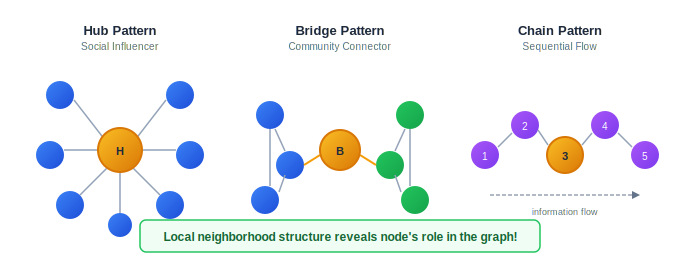
\includegraphics[width=0.65\textwidth]{img/graphs_examples_light.png}
\end{frame}

%-----------------------------------------------------------------------
\section{GraphSAGE Framework}
%-----------------------------------------------------------------------

\begin{frame}{GraphSAGE: Inductive Framework}
    \textbf{Core Principle:} Sample + Aggregate
    
    \vspace{10pt}
    \begin{itemize}
        \item Learn \textbf{aggregator functions} (not node embeddings)
        \item For any node $v$: \textbf{sample neighbors, aggregate their features}
        \item Pass through learned neural networks
        \item \textbf{Inference:} Apply same function to unseen nodes
    \end{itemize}
    
    \vspace{10pt}
    \centering
    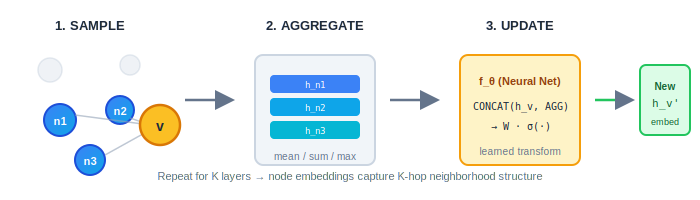
\includegraphics[width=0.95\textwidth]{img/graphsage_sample_aggregate_light.png}
\end{frame}

%-----------------------------------------------------------------------
\section{Implementation}
%-----------------------------------------------------------------------

\begin{frame}{Training GraphSAGE: The Challenge}
    \textbf{Dataset:} ogbn-products (Amazon co-purchase network)
    \begin{itemize}
        \item 2.4M nodes (products), 61M edges, 47 classes
        \item 8\% train / 2\% val / 90\% test split
    \end{itemize}

    \vspace{8pt}
    \textbf{The Problem:}
    \begin{itemize}
        \item Cannot fit entire graph in GPU memory
        \item Cannot do full message passing on 2.4M nodes
        \item \textbf{Solution:} Mini-batch training + neighbor sampling
    \end{itemize}
\end{frame}

\begin{frame}{Mini-Batch and Neighbor Sampling}
    \textbf{1. Mini-Batch Sampling:}
    \begin{itemize}
        \item Select small subset of seed nodes per iteration (e.g., 128 nodes)
        \item Only compute embeddings for these nodes + their neighborhoods
        \item Update model parameters based on batch loss
    \end{itemize}

    \vspace{8pt}
    \textbf{2. Neighbor Sampling (k-hop):}
    \begin{itemize}
        \item For each seed node, sample neighbors recursively for k layers
        \item \textbf{Fanout:} number of neighbors sampled per layer [L1, L2, ..., Lk]
        \item Example: [15, 10, 10, 10, 10] = 15 neighbors at layer 1, 10 at layers 2-5
    \end{itemize}

    \vspace{8pt}
    \textbf{Why this matters:}
    \begin{itemize}
        \item Fanout grows \textbf{exponentially}: $\sim$150k neighbors per seed node
        \item 128 seed nodes $\times$ 150k expansion = \textbf{19.2M nodes per batch}
        \item Memory bottleneck: sampled subgraphs >> model parameters
    \end{itemize}
\end{frame}

\begin{frame}{Neighbor Sampling: Visual Example}
    \begin{columns}
        \begin{column}{0.48\textwidth}
            \textbf{K-Hop Expansion:}
            \begin{itemize}
                \item Start with 1 seed node
                \item Sample neighbors recursively
                \item Fanout: [3, 2, 2] (simplified)
            \end{itemize}

            \vspace{8pt}
            \textbf{Growth per layer:}
            \begin{itemize}
                \item Layer 0: \textbf{1} seed
                \item Layer 1: 1 × 3 = \textbf{3}
                \item Layer 2: 3 × 2 = \textbf{6}
                \item Layer 3: 6 × 2 = \textbf{12}
            \end{itemize}
        \end{column}
        \begin{column}{0.48\textwidth}
            \centering
            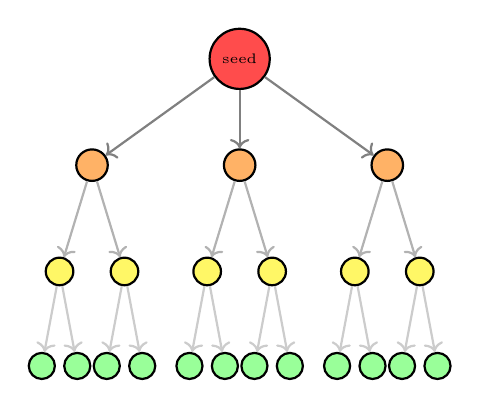
\begin{tikzpicture}[scale=0.75]
                % Layer 0 (seed)
                \node[circle, draw, thick, fill=red!70, minimum size=0.5cm] (s) at (0, 0) {\tiny seed};

                % Layer 1 (3 neighbors)
                \foreach \i in {1,2,3} {
                    \pgfmathsetmacro{\x}{(\i-2)*2.5}
                    \node[circle, draw, thick, fill=orange!60, minimum size=0.4cm] (n1\i) at (\x, -1.8) {};
                    \draw[->, thick, gray] (s) -- (n1\i);
                }

                % Layer 2 (6 neighbors - 2 per L1 node)
                \foreach \i in {1,2,3} {
                    \foreach \j in {1,2} {
                        \pgfmathsetmacro{\x}{(\i-2)*2.5 + (\j-1.5)*1.1}
                        \node[circle, draw, thick, fill=yellow!60, minimum size=0.35cm] (n2\i\j) at (\x, -3.6) {};
                        \draw[->, thick, gray!60] (n1\i) -- (n2\i\j);
                    }
                }

                % Layer 3 (12 neighbors - 2 per L2 node, only show some)
                \foreach \i in {1,2,3} {
                    \foreach \j in {1,2} {
                        \foreach \k in {1,2} {
                            \pgfmathsetmacro{\x}{(\i-2)*2.5 + (\j-1.5)*1.1 + (\k-1.5)*0.6}
                            \node[circle, draw, thick, fill=green!40, minimum size=0.25cm] (n3\i\j\k) at (\x, -5.2) {};
                            \draw[->, thick, gray!40] (n2\i\j) -- (n3\i\j\k);
                        }
                    }
                }
            \end{tikzpicture}
        \end{column}
    \end{columns}
\end{frame}

\begin{frame}{The Memory Explosion}
    \textbf{Real Configuration: [15, 10, 10, 10, 10]}

    \vspace{10pt}
    \centering
    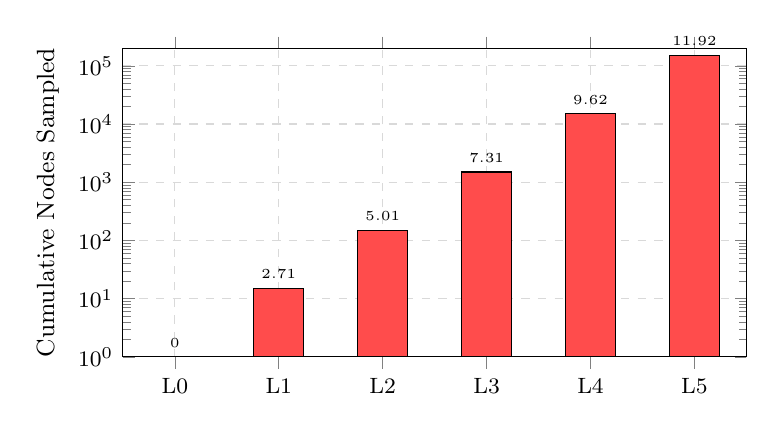
\begin{tikzpicture}
        \begin{axis}[
            ybar,
            symbolic x coords={L0, L1, L2, L3, L4, L5},
            xtick=data,
            ylabel={Cumulative Nodes Sampled},
            ymode=log,
            log origin=infty,
            width=9.5cm,
            height=5.5cm,
            bar width=18pt,
            ymin=1,
            ymax=200000,
            ylabel style={font=\small},
            xlabel style={font=\small},
            tick label style={font=\footnotesize},
            grid=major,
            grid style={dashed, gray!30},
            nodes near coords,
            every node near coord/.append style={font=\tiny, rotate=0, anchor=south}
        ]
        \addplot[fill=red!70] coordinates {
            (L0, 1)
            (L1, 15)
            (L2, 150)
            (L3, 1500)
            (L4, 15000)
            (L5, 150000)
        };
        \end{axis}
    \end{tikzpicture}

    \vspace{8pt}
    {\small \textbf{Combined:} 128 seed nodes × 150k neighbors = \textbf{19.2M nodes/batch}}
\end{frame}

\begin{frame}{Training Environment}
    \textbf{HPC Infrastructure:}
    \begin{itemize}
        \item \textbf{Cluster:} MeluXina (Luxembourg National Supercomputer)
        \item \textbf{GPUs:} Up to 4x NVIDIA A100 (40GB) per node
        \item \textbf{Framework:} PyTorch 2.1.2 + PyTorch Geometric
        \item \textbf{Containerization:} Apptainer/Singularity for reproducibility
    \end{itemize}

    \vspace{8pt}
    \textbf{Why Distributed Training?}
    \begin{itemize}
        \item Single GPU: limited batch size due to memory (sampled subgraphs $\sim$30-40GB)
        \item \textbf{Solution:} Distributed Data Parallel (DDP) across multiple GPUs
        \item Partition training data, synchronize gradients
    \end{itemize}
\end{frame}

\begin{frame}{System Architecture Diagram}
    \centering
    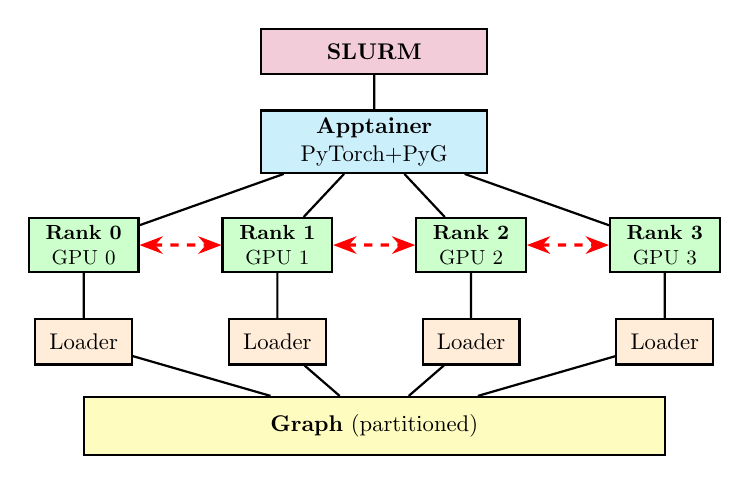
\begin{tikzpicture}[scale=0.82, every node/.style={transform shape}]

    % Styles
    \tikzset{
        boxstyle/.style={rectangle, draw, thick, minimum height=0.7cm, align=center},
        gpu/.style={boxstyle, fill=green!20, minimum width=1.7cm, font=\small},
        loader/.style={boxstyle, fill=orange!15, minimum width=1.5cm},
        graphbox/.style={boxstyle, fill=yellow!25, minimum width=9cm, minimum height=0.9cm},
        arrow/.style={-, >=Stealth, thick},
        redarrow/.style={<->, >=Stealth, very thick, red, dashed}
    }

    % Top layers
    \node[boxstyle, fill=purple!20, minimum width=3.5cm] (slurm) at (0, 5.2) {\textbf{SLURM}};
    \node[boxstyle, fill=cyan!20, minimum width=3.5cm] (container) at (0, 3.8) {\textbf{Apptainer}\\PyTorch+PyG};

    % GPU ranks
    \node[gpu] (r0) at (-4.5, 2.2) {\textbf{Rank 0}\\GPU 0};
    \node[gpu] (r1) at (-1.5, 2.2) {\textbf{Rank 1}\\GPU 1};
    \node[gpu] (r2) at (1.5, 2.2) {\textbf{Rank 2}\\GPU 2};
    \node[gpu] (r3) at (4.5, 2.2) {\textbf{Rank 3}\\GPU 3};

    % NCCL
    \draw[redarrow] (r0) -- (r1);
    \draw[redarrow] (r1) -- (r2);
    \draw[redarrow] (r2) -- (r3);

    % Loaders
    \node[loader] (l0) at (-4.5, 0.7) {Loader};
    \node[loader] (l1) at (-1.5, 0.7) {Loader};
    \node[loader] (l2) at (1.5, 0.7) {Loader};
    \node[loader] (l3) at (4.5, 0.7) {Loader};

    % Graph data
    \node[graphbox] (gdata) at (0, -0.6) {\textbf{Graph} (partitioned)};

    % Arrows
    \draw[arrow] (slurm) -- (container);
    \foreach \r in {r0,r1,r2,r3} {
        \draw[arrow] (container) -- (\r);
    }
    \foreach \i in {0,1,2,3} {
        \draw[arrow] (r\i) -- (l\i);
        \draw[arrow] (gdata) -- (l\i);
    }

    \end{tikzpicture}

    \vspace{3pt}
    {\footnotesize Multi-GPU DDP: data partitioned across 4 GPUs, gradients synced via NCCL}
\end{frame}

\begin{frame}{Containerization}
    \begin{itemize}
        \item \textbf{Base:} \texttt{pytorch/pytorch:2.1.2-cuda12.1-cudnn8-runtime}
        \item \textbf{Dependencies:} PyTorch Geometric, pyg-lib, OGB, torch-scatter/sparse
        \item \textbf{Why containerize?}
        \begin{itemize}
            \item Complex dependency graph (CUDA-compiled extensions)
            \item Reproducibility across HPC environments
            \item Avoid version conflicts on shared cluster
        \end{itemize}
    \end{itemize}
\end{frame}

\begin{frame}{Why HPC and Parallelism?}
    \textbf{1. Dimension of the Problem:}
    \begin{itemize}
        \item Each batch node samples 5-hop neighborhoods
        \item Fanout $\rightarrow$ exponential growth: $\sim$150k neighbors per seed node
        \item Batch 128 nodes $\times$ 150k expansion = 19.2M nodes per batch
    \end{itemize}

    \vspace{8pt}
    \textbf{2. Memory Bottleneck:}
    \begin{itemize}
        \item Model parameters: only $\sim$8 MB
        \item Sampled subgraphs + intermediate activations: \textbf{30-40 GB} per batch
        \item Single GPU cannot handle large batches $\rightarrow$ slow training
    \end{itemize}

    \vspace{8pt}
    \textbf{3. Solution: Data Parallelism with DDP}
    \begin{itemize}
        \item More GPUs with fixed batch size $\Rightarrow$ bigger effective batch size $\Rightarrow$ faster convergence
        \item \textbf{DeepSpeed overkill}
    \end{itemize}
\end{frame}

\begin{frame}{Distributed Data Parallel (DDP) Training}
    \begin{enumerate}
        \item \textbf{Process Initialization:}
        \begin{itemize}
            \item SLURM launches 4 processes (1 per GPU)
            \item Each process: independent Python interpreter + CUDA context
            \item NCCL backend for GPU-to-GPU communication
        \end{itemize}

        \vspace{4pt}
        \item \textbf{Data Partitioning:}
        \begin{itemize}
            \item Training set split across ranks (no overlap)
            \item Each rank: independent NeighborLoader for k-hop sampling
            \item 4-8 worker processes prefetch batches per GPU
        \end{itemize}

        \vspace{4pt}
        \item \textbf{Forward + Backward (Parallel):}
        \begin{itemize}
            \item Each GPU independently processes its batch
            \item Compute loss, backpropagate gradients
        \end{itemize}

        \vspace{4pt}
        \item \textbf{Gradient Synchronization:}
        \begin{itemize}
            \item DDP all-reduce: average gradients across all GPUs
            \item Optimizer step with synchronized gradients
        \end{itemize}
    \end{enumerate}
\end{frame}

%-----------------------------------------------------------------------
\section{Hyperparameters}
%-----------------------------------------------------------------------

\begin{frame}{Overview}
    \textbf{\faIcon{bullseye} Goal:} Scalable and reproducible hyperparameter optimization
    
    \vspace{8pt}
    \textbf{Model Architecture:} GraphSAGE (SAGEConv + LayerNorm + ReLU)

    \vspace{8pt}
    \textbf{Approach:}
    \begin{itemize}
        \item[\faIcon{box}] \textbf{Apptainer containers:}  reproducible environments
        \item[\faIcon{server}] \textbf{SLURM job arrays:} parallel execution across configs
        \item[\faIcon{file-csv}] \textbf{CSV-driven pipeline:} configuration \& result logging
    \end{itemize}

\end{frame}

\begin{frame}{Benchmark Pipeline}
    \centering
    \begin{tikzpicture}[scale=0.78, every node/.style={transform shape}]
    
    % Styles
    \tikzset{
        block/.style={rectangle, draw, thick, fill=blue!15, minimum width=2.2cm, minimum height=0.9cm, align=center, rounded corners=3pt},
        data/.style={rectangle, draw, thick, fill=yellow!25, minimum width=2cm, minimum height=0.7cm, align=center, rounded corners=2pt},
        arrow/.style={->, >=Stealth, thick, color=gray!70},
        label/.style={font=\scriptsize, align=center, color=gray!80}
    }
    
    % CSV Config
    \node[data] (csv) at (-5, 2) {\faIcon{file-csv} \texttt{hyperparams.csv}};
    
    % SLURM
    \node[block, fill=purple!20] (slurm) at (-5, 0) {\faIcon{server} \textbf{SLURM}\\Job Array};
    
    % Parallel jobs
    \node[block, fill=green!20, minimum width=1.5cm] (j0) at (-2, 1) {Job 0};
    \node[block, fill=green!20, minimum width=1.5cm] (j1) at (-2, 0) {Job 1};
    \node[block, fill=green!20, minimum width=1.5cm] (jn) at (-2, -1) {Job N};
    \node at (-2, 0.5) {$\vdots$};
    \node at (-2, -0.5) {$\vdots$};
    
    % Container + Training
    \node[block, fill=cyan!20, minimum width=2.5cm] (container) at (1.5, 0) {\faIcon{box} \textbf{Apptainer}\\DDP Training};
    
    % GPU box
    \node[block, fill=orange!20, minimum width=2cm] (gpu) at (4.8, 0) {\faIcon{microchip} 4× A100\\GPUs};
    
    % Results
    \node[data] (results) at (4.8, -2.5) {\faIcon{file-csv} \texttt{results.csv}};
    
    % Plotter
    \node[block, fill=magenta!20, minimum width=2cm] (plotter) at (1.5, -2.5) {\faIcon{python} \texttt{plotter.py}};
    
    % Output plots
    \node[data, fill=green!15] (plots) at (-2, -2.5) {\faIcon{chart-bar} \texttt{plot.png}};
    
    % Arrows
    \draw[arrow] (csv) -- (slurm);
    \draw[arrow] (slurm) -- (j0);
    \draw[arrow] (slurm) -- (j1);
    \draw[arrow] (slurm) -- (jn);
    \draw[arrow] (j0) -- (container);
    \draw[arrow] (j1) -- (container);
    \draw[arrow] (jn) -- (container);
    \draw[arrow] (container) -- (gpu);
    \draw[arrow] (gpu) -- (results);
    \draw[arrow] (results) -- (plotter);
    \draw[arrow] (plotter) -- (plots);
    
    % Lock annotation
    \node[label] at (6.5, -2.5) {\faIcon{lock}};
    
    \end{tikzpicture}
\end{frame}

\begin{frame}{Tunable Hyperparameters}
    \centering
    \small
    \begin{tabular}{@{} l l l l @{}}
    \toprule
    & \textbf{Parameter} & \textbf{Default} & \textbf{Range Tested} \\
    \midrule
    \faIcon{cubes} & \texttt{batch\_size} & 128 & 16--512 \\
    \faIcon{layer-group} & \texttt{accum\_steps} & 5 & 1--5 \\
    \faIcon{project-diagram} & \texttt{num\_neighbors} & [15,10,10,10,10] & various \\
    \midrule
    \faIcon{bars} & \texttt{num\_layers} & 5 & \textcolor{gray}{fixed} \\
    \faIcon{arrows-alt-h} & \texttt{hidden\_dim} & 256 & \textcolor{gray}{fixed} \\
    \faIcon{tachometer-alt} & \texttt{lr} & 0.003 & \textcolor{gray}{fixed} \\
    \faIcon{clock} & \texttt{epochs} & 150 & \textcolor{gray}{fixed} \\
    \faIcon{hourglass-half} & \texttt{patience} & 10 & \textcolor{gray}{fixed} \\
    \faIcon{random} & \texttt{dropout} & 0.5 & \textcolor{gray}{fixed} \\
    \bottomrule
    \end{tabular}
    
    \vspace{12pt}
    \begin{columns}
        \begin{column}{0.55\textwidth}
            {\footnotesize \faIcon{calculator} \textbf{Effective batch size:}}\\
            {\footnotesize \quad\texttt{batch\_size} $\times$ \texttt{accum\_steps} $\times$ \texttt{world\_size}}
        \end{column}
        \begin{column}{0.42\textwidth}
            {\footnotesize \faIcon{flask} \textbf{Configs tested:} 36}\\
            {\scriptsize \quad 16 batch $\cdot$ 16 neighbor $\cdot$ 4 scaling}
        \end{column}
    \end{columns}
\end{frame}

%-----------------------------------------------------------------------
\section{Results}
%-----------------------------------------------------------------------

\begin{frame}{Benchmarking Focus}

    \begin{enumerate}
        \item \textbf{Mini-batch sampling:} Batch size impact on time \& memory
        \vspace{0.3cm}
        \item \textbf{Neighbor sampling:} Fanout strategies (accuracy vs. efficiency)
        \vspace{0.3cm}
        \item \textbf{GPU scaling:} 1/2/4/8 GPU distributed training
    \end{enumerate}
\end{frame}

%-----------------------------------------------------------------------
\subsection{Mini-batch Sampling}
%-----------------------------------------------------------------------

\begin{frame}{Mini-batch Benchmarking: Configurations}
    \begin{columns}
        \begin{column}{0.6\textwidth}
            \textbf{What's being tested?}
            
            \vspace{8pt}
            How does \textbf{batch size} and \textbf{gradient accumulation} affect:
            \begin{itemize}
                \item Training time per epoch
                \item Peak GPU memory usage
                \item Overall training efficiency
            \end{itemize}
        \end{column}
        \begin{column}{0.4\textwidth}
            \footnotesize
            \begin{tabular}{|l|c|}
            \hline
            \textbf{Batch Size} & \textbf{Accum. Steps} \\
            \hline
            16 & 5 \\
            \hline
            32 & 5 \\
            \hline
            64 & 5 \\
            \hline
            64 & 1, 2, 3, 4 \\
            \hline
            \textbf{128} & \textbf{5} \\
            \hline
            128 & 1, 2, 3, 4 \\
            \hline
            160 & 5 \\
            \hline
            192 & 5 \\
            \hline
            256 & 5 \\
            \hline
            512 & 5 \\
            \hline
            \end{tabular}
        \end{column}
    \end{columns}
\end{frame}

\begin{frame}{Batch Size: Training Time}
    \begin{columns}
        \begin{column}{0.58\textwidth}
            \centering
            \includegraphics[width=\textwidth]{img/time_per_epoch_vs_batch_size.png}
        \end{column}
        \begin{column}{0.38\textwidth}
            \textbf{Key Findings:}
            \begin{itemize}
                \item Inverse relationship: larger batch = faster training
                \item Better GPU utilization with larger batches
                \item Reduced forward pass / backward pass overhead
            \end{itemize}
        \end{column}
    \end{columns}
\end{frame}

\begin{frame}{Batch Size: Memory Consumption}
    \begin{columns}
        \begin{column}{0.58\textwidth}
            \centering
            \includegraphics[width=\textwidth]{img/peak_memory_vs_batch_size.png}
        \end{column}
        \begin{column}{0.38\textwidth}
            \textbf{Key Findings:}
            \begin{itemize}
                \item \textbf{Max batch size:} 160
                \item Uses $\sim$32GB (7.5GB system overhead)
                \item Bigger batches go OOM
            \end{itemize}
        \end{column}
    \end{columns}
\end{frame}

%-----------------------------------------------------------------------
\subsection{Neighbor Sampling}
%-----------------------------------------------------------------------

\begin{frame}{Neighbor Sampling: Configurations}
    \begin{columns}
        \begin{column}{0.7\textwidth}
            \textbf{What's being tested?}
            
            \vspace{8pt}
            How do different \textbf{fanout strategies} affect:
            \begin{itemize}
                \item Test accuracy
                \item Training time per epoch
                \item GPU memory usage
            \end{itemize}
            
            \vspace{12pt}
            \textbf{Fanout} = neighbors sampled per layer\\
 
            \textbf{Total Fanout} = product across all layers
            $$F_{\text{total}} = \prod_{i=1}^{5} L_i$$
            

        \end{column}
        \begin{column}{0.3\textwidth}
            \tiny
            \begin{tabular}{|c|c|c|c|c|}
            \hline
            \textbf{L1} & \textbf{L2} & \textbf{L3} & \textbf{L4} & \textbf{L5} \\
            \hline
            50 & 0 & 0 & 0 & 0 \\
            \hline
            15 & 0 & 0 & 0 & 0 \\
            \hline
            15 & 10 & 0 & 0 & 0 \\
            \hline
            15 & 10 & 10 & 0 & 0 \\
            \hline
            15 & 10 & 10 & 10 & 0 \\
            \hline
            \textbf{15} & \textbf{10} & \textbf{10} & \textbf{10} & \textbf{10} \\
            \hline
            10 & 10 & 10 & 10 & 10 \\
            \hline
            12 & 12 & 12 & 12 & 12 \\
            \hline
            15 & 15 & 15 & 15 & 15 \\
            \hline
            20 & 15 & 10 & 5 & 3 \\
            \hline
            15 & 15 & 10 & 5 & 5 \\
            \hline
            15 & 15 & 15 & 5 & 5 \\
            \hline
            12 & 11 & 10 & 9 & 8 \\
            \hline
            5 & 5 & 5 & 5 & 5 \\
            \hline
            3 & 5 & 10 & 15 & 20 \\
            \hline
            30 & 10 & 5 & 3 & 3 \\
            \hline
            \end{tabular}
        \end{column}
    \end{columns}
\end{frame}

\begin{frame}{Neighbor Sampling: Accuracy vs. Time}
    \begin{columns}
        \begin{column}{0.58\textwidth}
            \centering
            \includegraphics[width=\textwidth]{img/neighbor_efficiency_time_vs_accuracy.png}
        \end{column}
        \begin{column}{0.38\textwidth}
            \textbf{Key Findings:}
            \begin{itemize}
                \item Upper-left = optimal
                \item Moderate fanouts best balance
                \item Aggressive sampling hurts accuracy or stability
                \item Very high fanouts: no proportional gains
            \end{itemize}
        \end{column}
    \end{columns}
\end{frame}

\begin{frame}{Neighbor Sampling: Memory vs. Fanout}
    \begin{columns}
        \begin{column}{0.58\textwidth}
            \centering
            \includegraphics[width=\textwidth]{img/neighbor_memory_vs_fanout.png}
        \end{column}
        \begin{column}{0.38\textwidth}
            \textbf{Key Findings:}
            \begin{itemize}
                \item Rapid memory growth with fanout
                \item Must balance receptive field vs. memory
                \item High fanouts hit memory limits and go OOM
            \end{itemize}
        \end{column}
    \end{columns}
\end{frame}

\begin{frame}{Top 5 Neighbor Configurations}
    \centering
    \small
    \begin{tabular}{|c|l|c|c|}
    \hline
    \textbf{Rank} & \textbf{Neighbor Sampling} & \textbf{Test Acc} & \textbf{Time (h)} \\
    \hline
    1 & [15, 15, 15, 5, 5] & 0.8121 & 14.56 \\
    \hline
    2 & [15, 10, 10, 10, 0] & 0.8114 & \textbf{7.22} \\
    \hline
    \textcolor{orange}{3} & \textcolor{orange}{[15, 10, 10, 10, 10]} & \textcolor{orange}{0.8096} & \textcolor{orange}{19.53} \\
    \hline
    4 & [10, 10, 10, 10, 10] & 0.8088 & 16.46 \\
    \hline
    5 & [20, 15, 10, 5, 3] & 0.8055 & 11.60 \\
    \hline
    \end{tabular}
    
    \vspace{10pt}
    
    {\footnotesize \textbf{Key insight:} [15,10,10,10,0] nearly matches accuracy, and \textbf{2.7× faster}}
\end{frame}

%-----------------------------------------------------------------------
\subsection{GPU Scaling}
%-----------------------------------------------------------------------

\begin{frame}{GPU Scaling: Configurations}
    \begin{columns}
        \begin{column}{0.5\textwidth}
            \textbf{What's being tested?}
            
            \vspace{8pt}
            How does \textbf{distributed training} scale across:
            \begin{itemize}
                \item 1/2/4 GPUs per node
                \item 4 GPUs across 2 nodes (8 GPUs total)
            \end{itemize}
            
        \end{column}
        \begin{column}{0.48\textwidth}
            \footnotesize
            \begin{tabular}{|l|l|}
            \hline
            \textbf{Configuration} & \textbf{Setup} \\
            \hline
            1 GPU & 1 node \\
            \hline
            2 GPUs & 1 node \\
            \hline
            4 GPUs & 1 node \\
            \hline
            8 GPUs & 2 nodes \\
            \hline
            \multicolumn{2}{|c|}{\textbf{Fixed Hyperparameters}} \\
            \hline
            Batch size & 128 \\
            \hline
            Neighbors & {[}15,10,10,10,10{]} \\
            \hline
            Epochs & 10 \\
            \hline
            \end{tabular}
        \end{column}
    \end{columns}
\end{frame}

\begin{frame}{GPU Scaling: Training Time}
    \begin{columns}
        \begin{column}{0.58\textwidth}
            \centering
            \includegraphics[width=\textwidth]{img/scaling_time_per_epoch.png}
        \end{column}
        \begin{column}{0.38\textwidth}
            \textbf{Key Findings:}
            \begin{itemize}
                \item \textbf{1→2 GPUs:}\\ 1.93× (96.5\% efficiency)
                \item \textbf{1→4 GPUs:}\\ 3.73× (93\% efficiency)
                \item \textbf{1→8 GPUs:}\\ 7.1× (89\% efficiency)

            \end{itemize}
        \end{column}
    \end{columns}
\end{frame}

\begin{frame}{GPU Scaling: Training Loss}
    \begin{columns}
        \begin{column}{0.58\textwidth}
            \centering
            \includegraphics[width=\textwidth]{img/scaling_train_loss.png}
        \end{column}
        \begin{column}{0.38\textwidth}
            \textbf{Key Findings:}
            \begin{itemize}
                \item Loss increases with more GPUs
                \item Cause: larger effective batch size
                \item Reduced gradient noise
            \end{itemize}
        \end{column}
    \end{columns}
\end{frame}

%-----------------------------------------------------------------------
\section{Discussion}
%-----------------------------------------------------------------------

\begin{frame}{Bottlenecks Discovered}
    \begin{itemize}
        \item \textbf{Memory wall:} Neighbor sampling expansion dominates memory usage
        \begin{itemize}
            \item Fanout [15,10,10,10,10] = 150k neighbors per seed node
            \item 128 batch size × 150k expansion = 19.2M nodes per batch
            \item Sampled subgraph + activations >> model parameters (8MB)
        \end{itemize}
        
        \vspace{6pt}
        \item \textbf{Inter-node communication:} InfiniBand NCCL all-reduce overhead
        \begin{itemize}
            \item 4 GPUs (1 node): 93\% efficiency
            \item 8 GPUs (2 nodes): 89\% efficiency (4\% degradation)
        \end{itemize}
        
        \vspace{6pt}
        \item \textbf{Loss convergence trade-off:} Larger effective batch sizes hurt convergence
        \begin{itemize}
            \item Training loss increases with GPU count
            \item Reduced gradient noise
        \end{itemize}
    \end{itemize}
\end{frame}

\begin{frame}{What Worked Well}
    \begin{itemize}
        \item \textbf{DDP implementation:} Seamless gradient synchronization across GPUs
        \begin{itemize}
            \item PyTorch DDP handles all-reduce automatically
            \item Minimal code changes from single-GPU baseline
        \end{itemize}
        
        \vspace{6pt}
        \item \textbf{Strong intra-node scaling:} Excellent up to 4 GPUs
        \begin{itemize}
            \item Linear speedups: 1→4 GPUs = 3.73× (93\% efficiency)
            \item PCIe/NVLink bandwidth sufficient for this dataset size
        \end{itemize}
        
        \vspace{6pt}
        \item \textbf{Containerization:} Reproducibility \& portability
        \begin{itemize}
            \item Apptainer/Singularity ensures consistent environment
            \item Complex PyG dependencies properly managed
        \end{itemize}
    \end{itemize}
\end{frame}


\begin{frame}{Lessons Learned}
    \textbf{Implementing High-Performance Systems:}
    
    \vspace{8pt}
    \begin{enumerate}
        \item \textbf{Profile first, optimize second:} Memory bound, not compute
        
        \vspace{4pt}
        \item \textbf{Trade-offs are everywhere:} No free lunch $\rightarrow$ accuracy, speed, memory, communication always compete
        
        \vspace{4pt}
        \item \textbf{Reproducibility matters:} Containerization and fixed seeds essential for scientific HPC work
        
    \end{enumerate}
\end{frame}


%-----------------------------------------------------------------------
\QApage

\bibliographpage

\end{document}
